\chapter{Analysis}
This chapter gives overview of two significant related platforms on which this work depends - Google Dapper and Zipkin. It continues with description of several background concepts and tools which are to some level relevant to the thesis, such as tools for large scale debugging, tools for visualizing the monitored data and also several profiling tools and their comparison. The libraries for bytecode instrumentation and different communication middle-wares are described in detail as the selected libraries affect the platform at very low level. This chapter ends with a comparison of different approaches to instrumenting Java applications.
\section{Related Work}
The most significant platforms to this thesis are Google Dapper and Zipkin, where Zipkin is based on the previous. Both serves the same core purpose which is to monitor large-scale Java based distributed applications. This thesis is based mainly on Google Dapper but also uses helpful Zipkin modules such as the user interface. Since Zipkin is developed according to Google Dapper design, these two platforms shares very similar concepts. The most important concept is a Span and it is explained in more details in the  following section. For now, we can think of a span as time slots encapsulating several calls from one node to another with well-defined start and end of the communication. The following two sections describes the basics the both mentioned platform. Both Zipkin and Dapper shares very similar concepts wo we just point out the most import parts relevant to the thesis.
\subsection{Google Dapper}
Google Dapper is proprietary software which was mainly developed as a tool for monitoring large distributed applications since debugging and reasoning about applications running on multiple host at the same time, sometimes written in different programming languages is inherently complex. Google Dapper has 3 main pillars on which is built:
\begin{itemize}
	\item Low overhead
	It was assumed that such a tool should share the same life-cycle as the monitored application itself thus low overhead was on of the main design goals as well. Google dapper 
	\item Application level transparency
	The developers and users of the application should not know about the monitoring tool and are not supposed to change the way how they interact with the system. It can be assumed from the paper that achieving application level transparency at Google was easier than it could be in more diverse environments since all the code produced in the Google shares the same libraries and control flow.
	\item Scalability
	Such a system should perform well on large scale data.
\end{itemize}	
Google Dapper collects so called distributed traces. The origin of the distributed trace is the communication/task initiator and the trace spans across the nodes in the cluster which took part as the computation/communication.
	
There were two proposals for obtaining this information - using the black-box and annotation-based monitoring approaches. The first one assumes no additional knowledge about the application whereas the second can use of additional information via annotations. Dapper is mainly using black-box monitoring schema since most of the control flow and RPC subsystems are shared among Google.
	
In Dapper, distributed traces are captured in so called trace trees, where tree nodes are basic units of work referred to as spans. Span is related to other spans via dependency edges. These edges represents relationship between parent span and children of this span. Usually the edges represents some kind of RPC calls or similar kind of communication.

Each span its own id so it can be uniquely identified. In order to reconstruct the whole trace tree, we need to be able to identify the starting Span. Spans without parent id are called root spans serves exactly that purpose. Span can also contain information from multiple hosts, usually from spans from direct neighborhood. Spans structure in Dapper platform is described in the figure \ref{fig:dapper_span}.
\begin{figure}
	\centering
		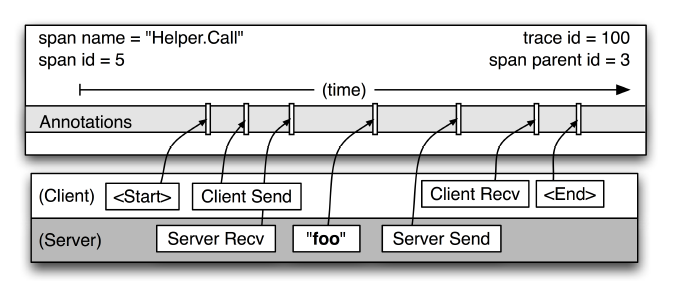
\includegraphics[scale=0.7]{dapper_span.png}
	\caption{Example of Span in Google Dapper. Picture taken from the Google Dapper paper}
	\label{fig:dapper_span}
\end{figure}

Dapper is able to achieve application-level transparency and follow distributed control paths thanks to instrumentation of a few common, mostly shared libraries among Google developers. 
\begin{itemize}
	\item Dapper attaches so called trace-context as thread-local variable to the thread when the thread handles any kind of control path. Trace context is small data structure containing mainly just reference to current and parent span via their ids.
	
	\item Dapper instruments the callback mechanism so when computation is deferred, the callbacks still carry around trace context of the creator and therefore also parent span ans current span id
	
	\item Most of the communication in Google is using single RPC framework with language bindings to different languages. This library was instrumented as well to achieve the desired transparency.
\end{itemize}

Even though Dapper is mainly following black-box monitoring scheme mentioned bellow, it still have small support for adding custom annotation to the code. This gives the developer of an application possibility to attach additional information to spans which are very application-specific.

The low-level overhead was also achieved by sampling the data. As is mentioned in the paper, the volume of data at Google is significant so only samples are taken at a time.

\subsection{Zipkin}
Zipkin is open-source distributed tracing system. It based on Google Dapper technical paper and manages both the collection and lookup of captured data.

Zipkin uses instrumentation and annotations for capturing the data. Some
information are captured automatically such as time when Span was created whereas some are optional and some even application-specific.

Zipkin architecture can bee seen on figure \ref{fig:zipkin_architecture}.
\begin{figure}
	\centering
	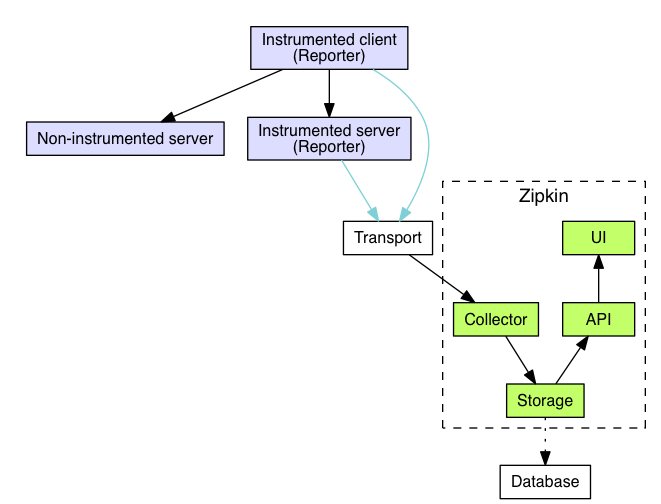
\includegraphics[scale=0.7]{zipkin_architecture.png}
	\caption{Zipkin architecture - http://zipkin.io/pages/architecture.html}
	\label{fig:zipkin_architecture}
\end{figure}
The instrumented application is responsible for creating valid traces. For that reason Zipkin has set of pre-instrumented libraries ready to be used which works well with whole Zipkin infrastructure. Spans are stored asynchronously in Zipkin to ensure lower overhead.

Once the span is created, it is sent to Zipkin, in more details, to Zipkin collector. In General, Zipkin consists of 4 components:
\begin{itemize}
	\item Zipkin Collector
	It is usually a daemon thread or process which stores, validates and indexes the data for future lockups.
	\item Storage
	Data in zipkin can be stored in a mulltiple ways, so this is a pluggable component. Data can be stored in for example in Cassandra, MySQL or can be send to Zipkin UI right away without storing it anywhere. The last option is good only for small amount of data.
	\item Zipkin Query Service
	This component act as a query daemon allowing us to query various informaion about span using simple JSON API.
	\item Web UI
	Basic, but very useful user interface. The user can see whole trace trees and all spans with dependencies between them.
\end{itemize}
 In the thesis the Zipkin UI is used as front end for developed the monitoring tool and it's format is described in more detail in  \hyperref[sec:zipkin_ui]{Zipkin UI} section of \hyperref[chap:design]{Design} chapter.
 
 The reason why Zipkin UI was selected as the primary user interface for this work is mainly it's simplicity and ease of use. Also it fulfills the visualization requirements of the thesis as well, since we need to see dependencies between spans and also whole trace tree as well. However the monitoring platform is not tightly-coupled with this user interface. We will see later how to create custom span savers which can store data in any format suitable for different visualization tools.
 
\section{Background and Tools}
\subsection{Tools for Large-Scale Debugging}
\subsection{Tools for Visualizations the Captured Data}
\subsubsection{Flame Charts}
\subsubsection{Graphite and Graphana}
\subsection{Profiling Tools}
\subsubsection{System Profilers}
\subsubsection{JVM Profilers}
Write about AsyncGetCallTrace



\section{Instrumentation Libraries}
\subsection{Javassist}
\subsection{ByteBuddy}
\subsection{CGlib}
\subsection{ASM}
.. just give brief overview what were the instrumentation libreries choices. The selected one will be describied in the next section

\section{Communication Middleware}
give comparison between the possible communication middle-wares
\subsection{Raw Sockets}
\subsection{ZeroMQ}
\subsection{NanoMSG}

\section{Comparison of Agent Approaches}
give introduction to various instrumentation techniques and compare the 2 approaches
\subsection{Java Agent Solution}
\subsection{Native Agent Solution}

